\documentclass[aspectratio=169,10pt]{beamer}

\usetheme[block=fill,progressbar=foot,background=light]{metropolis}   
\setbeamercolor{background canvas}{bg=white}
\usepackage{appendixnumberbeamer}

\title{Introduction au DevOps}
\subtitle{Terraform}
\date{12 Septembre 2025}
\author{Jolan PHILIPPE}
\institute{Université d'Orléans}

\usepackage{graphicx}
%\usepackage{cite}
\usepackage{subcaption}
\usepackage{lmodern}
\usepackage{hyperref}
\usepackage{array}
\usepackage{multirow}
%\usepackage[table]{xcolor}
\usepackage{mathabx}
\usepackage{amsmath}
\usepackage{amssymb}
\usepackage{wrapfig}
\usepackage{fancyhdr}
\usepackage{url}
\usepackage{listings}
\usepackage{minted}
\usepackage{fontawesome}
\usepackage{tikz}
\usepackage{hyperref}
\usetikzlibrary{automata, positioning, matrix, fit}
\usetikzlibrary{arrows.meta,calc,decorations.markings,math}
\usetikzlibrary{shadows.blur}
\usetikzlibrary{decorations.pathreplacing, fit}
\usetikzlibrary{shapes,arrows}
\usepackage{flushend}
\usepackage{ifthen}
\newboolean{showtodos}

% ----------------------------------------
% COLORS
\definecolor{gray}{rgb}{0.5,0.5,0.5}
\definecolor{ashgrey}{rgb}{0.7, 0.75, 0.71}
\definecolor{battleshipgrey}{rgb}{0.52, 0.52, 0.51}
\definecolor{aliceblue}{rgb}{0.94, 0.97, 1.0}
\definecolor{mauve}{rgb}{0.58,0,0.82}
\definecolor{auburn}{rgb}{0.43, 0.21, 0.1}
\definecolor{babyblue}{rgb}{0.54, 0.81, 0.94}
\definecolor{amaranth}{rgb}{0.9, 0.17, 0.31}
\definecolor{bleudefrance}{rgb}{0.19, 0.55, 0.93}
\definecolor{atomictangerine}{rgb}{1.0, 0.6, 0.4}
\definecolor{beaublue}{rgb}{0.74, 0.83, 0.9}
\definecolor{dkviolet}{rgb}{0.9, 0.17, 0.31}
\definecolor{dkgreen}{rgb}{0.0, 0.42, 0.24}
\definecolor{ltblue}{rgb}{0.0, 0.75, 1.0}
\definecolor{dkblue}{rgb}{0.2, 0.2, 0.6}
\definecolor{dkred}{rgb}{0.8, 0.0, 0.0}
\definecolor{byzantine}{rgb}{0.74, 0.2, 0.64}
% ----------------------------------------



\usepackage[textwidth=17mm]{todonotes}
\newcommand{\instructions}[1]{
	\todo[color=black!20,inline,size=\small]{#1}
}
\newcommand{\customtodo}[4]{
\ifthenelse{\boolean{showtodos}} { 
	\todo[color=#2,inline,size=\small]{
		\ifx&#3&
		\textbf{#1} #4
		\else
		\textbf{#1$\Rightarrow$#3} #4
		\fi
	}
 } 
}{}

\newcommand{\jolan}[2][]{\customtodo{Jolan}{pink!40}{#1}{#2}}
\newcommand{\antoine}[2][]{\customtodo{Antoine}{red!40}{#1}{#2}}
\newcommand{\helene}[2][]{\customtodo{Helene}{orange!40}{#1}{#2}}
\newcommand{\issam}[2][]{\customtodo{Issam}{green!40}{#1}{#2}}
\newcommand{\charles}[2][]{\customtodo{Charles}{blue!40}{#1}{#2}}

\newcommand{\tmp}[1][]{\customtodo{To remove}{gray}{#1}}

\usepackage{xspace}
\newcommand{\ie}[0]{{\em i.e.},\xspace}
\newcommand{\vs}[0]{{\em vs.}\xspace}
\newcommand{\eg}[0]{{\em e.g.},\xspace}
\newcommand{\etal}[0]{{\em et al.}\xspace}
\newcommand{\wrt}[0]{{\em w.r.t.}\xspace}
\newcommand{\aka}[0]{{\em a.k.a.}\xspace}
\newcommand{\via}[0]{{\em via}\xspace}

% ----------------------------------------

\lstdefinestyle{goalstyle}{
  basicstyle=\scriptsize\itshape,
  xleftmargin=1em,
  literate={::=}{$::=$}{2},
  keywords={behaviors,ports,components,forall,component,behavior,port,status}
}

\lstdefinelanguage{MiniZinc}{
numberstyle=\tiny\color{gray},
% Anything betweeen $ becomes LaTeX math mode
mathescape=true,
% Comments may or not include Latex commands
texcl=false,
% Vernacular commands
morekeywords=[1]{ann, annotation, any, array, assert,
        bool,
        constraint,
        else, elseif, endif, enum, exists,
        float, forall, function,
        if, in, include, int,
        list,
        minimize, maximize,
        of, op, output,
        par, predicate,
        record,
        set, solve, string,
        test, then, tuple, type,
        var,
        where,
        %% MiniZinc functions
        %%
        abort, abs, acosh, array_intersect, array_union,
        array1d, array2d, array3d, array4d, array5d, array6d, asin, assert, atan,
        bool2int,
        card, ceil, combinator, concat, cos, cosh,
        dom, dom_array, dom_size, dominance,
        exp,
        fix, floor,
        index_set, index_set_1of2, index_set_2of2, index_set_1of3, index_set_2of3, index_set_3of3,
        int2float, is_fixed,Yaml
        join,
        lb, lb_array, length, let, ln, log, log2, log10,
        min, max,
        pow, product,
        round,
        set2array, show, show_int, show_float, sin, sinh, sqrt, sum,
        tan, tanh, trace,
        ub, and ub_array,
        %% Search keywords
        bool_search, int_search, seq_search, priority_search,
        %% MiniSearch keywords
        minisearch, search, while, repeat, next, commit, print, post, sol, scope, time_limit, break, fail},
numbers=left,
% Gallina
morekeywords=[2]{Array},
% Spaces are not displayed as a special character
showstringspaces=false,
% String delimiters
morestring=[b]",
morestring=[d]',
% Size of tabulations
tabsize=2,
% Enables ASCII chars 128 to 255
extendedchars=false,
% Case sensitivity
sensitive=true,
% Automatic breaking of long lines
breaklines=false,
% Default style fors listings
basicstyle=\footnotesize,
% Position of captions is bottom
captionpos=b,
% flexible columns
basewidth={2em, 0.5em},
columns=[l]flexible,
% Style for (listings') identifiers
identifierstyle={\ttfamily\color{black}},
% Style for declaration keywords
keywordstyle=[1]{\ttfamily\bfseries\color{dkviolet}},
% Style for gallina keywords
keywordstyle=[2]{\ttfamily\bfseries\color{dkgreen}},
% Style for strings
stringstyle=\ttfamily,
% Style for comments
commentstyle={\ttfamily\itshape\color{dkgreen}},
%moredelim=**[is][\ttfamily\color{red}]{/&}{&/},
literate=
  {forall}{{\color{dkgreen}{$\forall$}}}1
{exists}{{$\exists$}}1
{<-}{{$\leftarrow$}}1
{=>}{{$\Rightarrow$}}1
%{==}{{\code{==}}}1
%{==>}{{\code{==>}}}1
%    {:>}{{\code{:>}}}1
{->}{{$\rightarrow$}}1
{<-->}{{$\longleftrightarrow$}}1
{<->}{{$\leftrightarrow$}}1
{<==}{{$\leq$}}1
{\#}{{$^\star$}}1
{\\o}{{$\circ$}}1
%    {\@}{{$\cdot$}}1 
{\/\\}{{$\wedge$}}1
{\\\/}{{$\vee$}}1
%{++}{{\code{++}}}1
{~}{{\ }}1
{\@\@}{{$@$}}1
{\\mapsto}{{$\mapsto$}}1
{\\hline}{{\rule{\linewidth}{0.5pt}}}1
%
}[keywords,comments,strings]
\lstdefinestyle{mznstyle}{
  language=MiniZinc,
}
% ----------------------------------------
\lstdefinelanguage{MyPython}{
morekeywords=[1]{def, if, while, return, not},
morekeywords=[5]{get_messages, infer_constraints, plan_inference, infer_messages, bhv_inference, send_messages, allAcked, send_ack, ack, global_ack},
keywordstyle=[5]{\ttfamily\bfseries\color{purple}},
tabsize=2,
numbers=left,
numberstyle=\tiny\color{gray},
breaklines=true,
basicstyle=\footnotesize,
% literate= 
% {act_c}{{$act_c$}}1
% {Gbhv}{{$\Gamma bhv$}}1
% {Gfinal}{{$\Gamma final$}}1,
% {Gbhv_c}{{$\Gamma bhv_{c}$}}1
% {Gport_c}{{$\Gamma port_{c}$}}1
% {Gfinal_c}{{$\Gamma final_{c}$}}1
}
\lstdefinestyle{pythonstyle}{language=MyPython}
\lstMakeShortInline[language=MyPython]"

\newfloat{Model}{t}{lom}
\newcommand{\constraint}[1]{\textnormal{\textsc{#1}}}
\newcommand{\Regular}{\constraint{Regular}}
\newcommand{\CostRegular}{\constraint{CostRegular}}
\newcommand{\Count}{\constraint{Count}}
\newcommand{\Element}{\constraint{Element}}
\newcommand{\Sum}{\constraint{Sum}}

%------------------------------------------------------
\definecolor{codegreen}{rgb}{0,0.6,0}
\definecolor{codegray}{rgb}{0.5,0.5,0.5}
\definecolor{codepurple}{rgb}{0.58,0,0.82}
\definecolor{backcolour}{rgb}{0.95,0.95,0.92}
\lstdefinestyle{mystyle}{
    commentstyle=\color{codegreen},
    keywordstyle=\color{purple},
    tabsize=2,
    numbers=left,
    numberstyle=\tiny\color{gray},
    stringstyle=\color{codepurple},
    breaklines=true,
    basicstyle=\tiny
}


\definecolor{keywords}{RGB}{255,0,90}
\definecolor{comments}{RGB}{0,0,113}
\definecolor{red}{RGB}{160,0,0}
\definecolor{green}{RGB}{0,150,0}
\definecolor{backcolour}{rgb}{0.95,0.95,0.95}
\DeclareCaptionFont{white}{\color{white}}
\DeclareCaptionFont{gray}{\color{gray}}
\DeclareCaptionFormat{listing}{\colorbox{backcolour}{\parbox{\linewidth}{#1#2#3}}}
\captionsetup[lstlisting]{format=listing}%,labelfont=white,textfont=white}
\lstdefinestyle{mystyle}{
    tabsize=2,
    numberstyle=\tiny\color{gray},
    breaklines=true,
    numbers=left,
    backgroundcolor=\color{white},
    numbersep=5pt,
    keywordstyle=\color{keywords},
    commentstyle=\color{comments},
    stringstyle=\color{blue},
    showstringspaces=false,
    identifierstyle=\color{green},
    basicstyle=\scriptsize\ttfamily,
    numberstyle=\tiny\color{gray},
}

\lstdefinestyle{mysmallstyle}{
    tabsize=2,
    numberstyle=\tiny\color{gray},
    breaklines=true,
    numbers=left,
    backgroundcolor=\color{white},
    numbersep=5pt,
    keywordstyle=\color{keywords},
    commentstyle=\color{comments},
    stringstyle=\color{blue},
    showstringspaces=false,
    identifierstyle=\color{green},
    basicstyle=\scriptsize\ttfamily,
    numberstyle=\tiny\color{gray},
}

\lstdefinestyle{yaml}{
     basicstyle=\color{black}\scriptsize,
     keywords =[1]{behaviors, components, connections},
    keywordstyle=[1]{\color{blue}\scriptsize}, 
     rulecolor=\color{black},
     string=[s]{'}{'},
     stringstyle=\color{blue},
     comment=[l]{:},
     commentstyle=\color{black},
     morecomment=[l]{-}
 }

\usepackage{pifont,utfsym}
\newcommand{\cmark}{\ding{51}}
\newcommand{\xmark}{\ding{55}}
\newcommand{\OKmark}{{\color{green}\cmark}}
\newcommand{\KOmark}{{\color{red}\xmark}}



% \usetikzlibrary{positioning, arrows.meta, decorations.pathreplacing, fit}
% \pgfarrowsdeclare{lollipop}{lollipop}{
%     \pgfsetlinewidth{0.7pt}
%     \pgfarrowsleftextend{0pt}
%     \pgfarrowsrightextend{2pt}
% }{
%     \pgfpathcircle{\pgfpoint{0pt}{0pt}}{2pt}
%     \pgfusepathqfillstroke
% }
% \pgfarrowsdeclare{socket}{socket}{
%     \pgfarrowsleftextend{2pt}
%     \pgfarrowsrightextend{2pt}
% }{
%     \pgfsetlinewidth{0.7pt}
%     \pgfpathmoveto{\pgfqpoint{3pt}{-3pt}}
%     \pgfpatharc{270}{90}{3pt}
%     \pgfusepathqstroke
% }

% % Define styles for lollipop and socket arrows
% \tikzset{
%   lollipop/.style={
%     -{lollipop}
%   },
%   socket/.style={
%     -{socket}
%   }
% }





% Define a new arrow tip for the lollipop (filled circle)
\pgfarrowsdeclare{lollipop}{lollipop}{
    \pgfsetlinewidth{0.7pt}
    \pgfarrowsleftextend{0pt}
    \pgfarrowsrightextend{2pt}
}{
    \pgfpathcircle{\pgfpoint{0pt}{0pt}}{2pt}
    \pgfusepathqfillstroke
}

% Define a new arrow tip for the socket (reversed C)
\pgfarrowsdeclare{socket}{socket}{
    \pgfarrowsleftextend{2pt}
    \pgfarrowsrightextend{2pt}
}{
    \pgfsetlinewidth{0.7pt}
    \pgfpathmoveto{\pgfqpoint{3pt}{-3pt}}
    \pgfpatharc{270}{90}{3pt}
    \pgfusepathqstroke
}

% Define styles for lollipop and socket arrows
\tikzset{
  lollipop/.style={
    -{lollipop}
  },
  socket/.style={
    -{socket}
  }
}

\newcommand{\simpleprovideuse}[3][1cm]{%
    \path (#2) -- (#3) coordinate[pos=0.5] (mid#2#3);
    \draw[-{lollipop}] (#2) -- (mid#2#3);
    \draw[-{socket}] (#3) -- (mid#2#3);
}

\newcommand{\provideuse}[3][1cm]{
    % Usage :
    %   \provideuse{src}{target}
    % Example:
    %   \node[draw, circle] (A) {A};
    %   \node[draw, circle] (B) {B};
    %   \provideuse{A}{B}
    \path (#2) -- (#3) coordinate[pos=0.5] (mid#2#3);
    \path (#2) -- (mid#2#3) coordinate[pos=0.5] (q1#2#3);
    \path (mid#2#3) -- (#3) coordinate[pos=0.5] (q3#2#3);
    \draw[-{lollipop}] (#2) -- (q1#2#3);
    \draw[-{lollipop}] (mid#2#3) -- (q3#2#3);
    \draw[-{socket}] (#3) -- (q3#2#3);
    \draw[-{socket}] (q3#2#3) -- (q1#2#3);
}

\newcommand{\provideusetwolabels}[5][1cm]{%
    % Usage :
    %   \provideusetwolabels{src}{target}
    % Example:
    %   \node[draw, circle] (A) {A};
    %   \node[draw, circle] (B) {B};
    %   \provideusetwolabels{A}{B}{provide}{use}
    \path (#2) -- (#3) coordinate[pos=0.5] (mid#2#3);
    \path (#2) -- (mid#2#3) coordinate[pos=0.5] (q1#2#3);
    \path (mid#2#3) -- (#3) coordinate[pos=0.5] (q3#2#3);
    \draw[-{lollipop}] (#2) --  node[midway, above, xshift=0.08cm] {\tiny #4} (q1#2#3);
    \draw[-{lollipop}] (mid#2#3) -- (q3#2#3);
    \draw[-{socket}] (#3) -- node[midway, below, xshift=-0.4cm] { \tiny #5} (q3#2#3);
    \draw[-{socket}] (q3#2#3) -- (q1#2#3);
}

\newcommand{\provideusesinglelabel}[4][1cm]{%
    % Usage :
    %   \provideusesinglelabel{src}{target}
    % Example:
    %   \node[draw, circle] (A) {A};
    %   \node[draw, circle] (B) {B};
    %   \provideusesinglelabel{A}{B}{relation}
    \path (#2) -- (#3) coordinate[pos=0.5] (mid#2#3);
    \path (#2) -- (mid#2#3) coordinate[pos=0.5] (q1#2#3);
    \path (mid#2#3) -- (#3) coordinate[pos=0.5] (q3#2#3);
    \draw[-{lollipop}] (#2) -- (q1#2#3);
    \draw[-{lollipop}] (mid#2#3) -- (q3#2#3);
    \draw[-{socket}] (#3) -- (q3#2#3);
    \draw[-{socket}] (q3#2#3)  -- node[midway, above] {\scriptsize #4} (q1#2#3);
}

\usepackage{pifont,utfsym}
\newcommand{\cmark}{\ding{51}}
\newcommand{\xmark}{\ding{55}}
\newcommand{\okmark}{\textbf{\color{green}\faCheck}}
\newcommand{\komark}{\textbf{\color{red}\faTimes}}
\newcommand{\midmark}{\textbf{\color{orange}$\sim$}}
\renewcommand{\OKmark}{\okmark~}
\newcommand{\OKOKmark}{\okmark\okmark~}
\renewcommand{\KOmark}{\komark~}
\newcommand{\MIDmark}{\midmark~}

\begin{document}

\begin{frame}
    \titlepage 
\end{frame}
% -----------------

\begin{frame}{Les rôles des outils d'IaC}

\hspace*{-0.7cm}
\begin{tikzpicture}

    % \node[] (commit) {Commit Code};

\node[] (packaging) {
    \begin{tabular}{c}
    \textbf{Management}\\
    \textbf{d'application}
    \end{tabular}
    };
\node[below=0cm of packaging] (packagingL) {
    \begin{tabular}{c}
    \small Customiser, configurer\\
    \small tester l'application\\
    \small et la conteneuriser\\
    \small 
    \end{tabular}
};
\node[right=0.8cm of packaging] (provisioning) {
    \begin{tabular}{c}
    \textbf{Provisionnement} \\ 
    \textbf{d'infrastructure}
    \end{tabular}
};
\node[below=0cm of provisioning] (provisioningL) {
    \begin{tabular}{c}
    \small Demander ressources\\
    \small physiques ou virtuelles;\\
    \small configurer le réseau;\\
    \small et règles sécurité
    \end{tabular}
};
    
\node[right=0.8cm of provisioning] (configmanagement) {
    \begin{tabular}{c}
    \textbf{Installation et}\\
    \textbf{Configuration}
    \end{tabular}
};
\node[below=0cm of configmanagement] (configmanagementL) {
    \begin{tabular}{c}
    \small Installer les services\\
    \small (app + deps)\\
    \small configurer les services;\\
    \small et les intégrer
    \end{tabular}
};

    % -------

\node[right=0.8cm of configmanagement] (orchestration) {
\begin{tabular}{c}
\textbf{Orchestration}\\
\textbf{de cycle de vie}
\end{tabular}
};
\node[below=0cm of orchestration] (orchestrationL) {
\begin{tabular}{c}
\small Upgrades auto;\\
\small Backup et recovery;\\
\small Surveillance;\\
\small Passage à l'échelle
\end{tabular}
};

\node[rectangle, draw, fit=(provisioning) (provisioningL), dkblue, line width=2pt](){};
    
\end{tikzpicture}

\end{frame}

% -----------------
\section{Une infrastructure, c'est quoi ?}
% -----------------

\begin{frame}{Définitions}

\begin{alertblock}{Infrastructure}
L'infrastructure fait référence au logiciel, à la plate-forme ou au matériel qui fournit ou déploie des applications. \textit{Source: Infrastructure-as-code, patterns and practices}
\end{alertblock}

\begin{alertblock}{Infrastructure as a Service (IaaS)}
L’IaaS (infrastructure as a service) est un service de cloud computing offrant des ressources informatiques matérielles (stockage, réseau, baies de serveurs). \textit{Source: CNIL}
\end{alertblock}
    
\end{frame}

% -----------------

\begin{frame}{Dans le Cloud: Infrastructure $\Rightarrow$ APIs}

Dans un contexte de IaaS, le paradigme du Cloud computing a transformé l'\alert{infrastructure en APIs externes} (e.g., REST) sur lesquelles on peut envoyer des requêtes.

Aujourd'hui, dans le Cloud, les infrastructures sont comme n'importe quel logiciel offrant des services.
\begin{itemize}
    \item Une requête pour un bucket pour stocker du contenu (e.g., BDD)
    \item Une requête pour un cluster GKE (Google Kubernetes Engine) pour acquerir des applciations micro-services
    \item Une requête pour des machines virtuelles, sur lesquelles on installera une application ou des logiciels
    \item etc.
\end{itemize}
    
\end{frame}

% -----------------

\begin{frame}{Exemple}

\begin{center}
    \begin{tikzpicture}
    \node[draw, rectangle, minimum height=1cm, minimum width=2cm](bucket){Bucket};
    
    \node[draw, rectangle, minimum height=1cm, minimum width=2cm, right=1.2cm of bucket,yshift=0.8cm](bucketPublic){\begin{tabular}{c}Bucket Object\\PUBLIC\end{tabular}};
    
    \node[draw, rectangle, minimum height=1cm, minimum width=2cm, right=1.2cm of bucket,yshift=-0.8cm](bucketSensitive){\begin{tabular}{c}Bucket Object\\SENSITIVE\end{tabular}};

    
    \node[draw, rectangle, minimum height=1cm, minimum width=2cm, right=5cm of bucket](network){Network};
    
    \node[draw, rectangle, minimum height=1cm, minimum width=2cm, below=1cm of bucket](iam){\begin{tabular}{c}IAM\\Policy\end{tabular}};
    
    \node[draw, rectangle, minimum height=1cm, minimum width=2cm, above=1cm of bucket](backend){\begin{tabular}{c}Backend\end{tabular}};

    \simpleprovideuse{bucket}{backend}
    \simpleprovideuse{bucket}{iam}
    \simpleprovideuse{iam}{bucketSensitive}
    \simpleprovideuse{bucket}{bucketPublic}
    \simpleprovideuse{bucket}{bucketSensitive}
    \simpleprovideuse{network}{bucketSensitive}
    \simpleprovideuse{network}{bucketPublic}
    
\end{tikzpicture}
\end{center}
\end{frame}

% -----------------
\begin{frame}{Provisionner une infrastructure}

Les outils de provisionnement ont été fait pour rendre plus réutilisable, reproductible, flexible et sûr la gestion d'infrastructure dans le Cloud.

\begin{alertblock}{Solution spécifique}
\begin{itemize}
    \item Heat pour OpenStack
    \item Cloud Formation (CFN) pour Amazon Web Service (AWS)
    \item Azure Resource Manager (ARM) pour Microsoft Azure 
    \item GCP pour Google Cloud (déprécié, Google utilise maintenant Terraform)
\end{itemize}
\end{alertblock}

\begin{alertblock}{Solution multi-Cloud}
\begin{itemize}
    \item Terraform
    \item Pulumi
\end{itemize}
\end{alertblock}

\end{frame}

% -----------------
\begin{frame}{Provisionner une infrastructure}

\begin{alertblock}{Définition}
Le provisionnement est l'opération de création et de gestion d'un ensemble de ressources dans une infrastructure dans un Cloud public, un data center, ou solution de monitoring hébergée.
\end{alertblock}

Concrètement, le provisionnement c'est demander des machines et des ressources.

\pause

\begin{alertblock}{Ressources}
Dans le provisionnement, TOUT est une ressource. 
\begin{itemize}
    \item Une machine virtuelle
    \item Un stockage (e.g., BDD, services de stockage, etc.)
    \item Un réseau
    \item Un secret manager
    \item etc.
\end{itemize}
\end{alertblock}

\end{frame}

% -----------------
\begin{frame}{Terraform}

Dans ce module, nous utiliserons un outil de provisionnement: Terraform

\begin{center}

\includegraphics[scale=0.4]{images/terraform.png}
\end{center}

Terraform est un outil

\begin{itemize}
    \item \alert{Déclaratif}: l'état souhaité est décrit dans un fichier, en utilisant le langage \alert{HCL} (HashiCorp Configuration Language). 
    \item \alert{Stateful}: l'état courant de l'infrastructure est conservé dans un fichier. 
    \item De \alert{reconciliation}: l'état souhaité est comparé avec l'état courant pour définir quelle opérations (CRUD) doivent être réalisées. Ces actions sont ensuite exécutées. 
    \item \alert{Conccurent}: les opérations de réconcialtion peuvent être exécutée en parallel, tant que les dépendences sont respectées. 
\end{itemize}

\end{frame}
% -----------------
\begin{frame}{Boucle de reconciliation}
\begin{tikzpicture}[auto, node distance=1cm, scale=0.5]

% DevOps fig + txt
\node[yshift=0.5cm] (ldevops) {\LARGE \faMale};
\node[left=-0.1cm of ldevops] (rdevops) {\LARGE \faFemale};
\node[fit=(ldevops) (rdevops), inner sep=1pt] (sdevops) {};
\node[below=0 of sdevops] (devops) {DevOps};
\node[fit=(sdevops) (devops), inner sep=1pt] (blockdevops) {};

% Conflang
\node[draw, rectangle, rounded corners=5pt, right=1.3cm of blockdevops] (conflang) {\begin{tabular}{c}Language de\\configuration (HCL)\end{tabular}};
\node[above=-0.25cm of conflang, xshift=18pt](midconflang){};

% Target and current infra
\node[draw, rectangle, right=1.5cm of conflang, minimum height=1.4cm] (targetinfra) {\begin{tabular}{c}
Infrastructure\\Ciblée\end{tabular}};
\node[draw, rectangle, right=0.5cm of targetinfra, minimum height=1.4cm] (currentinfra) {\begin{tabular}{c}
Infrastructure\\Courante
\end{tabular}};
\node[fit=(targetinfra) (currentinfra), inner sep=1pt] (blockinfra) {};

% Ressources

% Reconciliation
\node[draw, rectangle, rounded corners=10pt, below=0.8cm of blockinfra] (reconciliation){\begin{tabular}{l}
Réconciliation d'état \\ 
$\bullet$ Différence \\ 
$\bullet$ Planifie la reconf. \\ 
$\bullet$ Exécute
\end{tabular}};

% New infra
\node[draw, rectangle, left=1.3cm of reconciliation, minimum height=0.7cm, minimum width=2cm] (newinfra) {\begin{tabular}{c}
Nouvelle\\Infrastructure
\end{tabular}};


% Arrows
\draw[-{Stealth[length=2mm]}, thick, line width=0.4mm] (blockdevops) -- node {utilise} (conflang);
\draw[-{Stealth[length=2mm]}, thick, line width=0.4mm] (conflang) -- node [above] {décrit} (targetinfra);

% \draw[-{Stealth[length=2mm]}, thick, line width=0.4mm] (conflang.north) -- node [below] {dirige, modifie} (currentinfra.north);

% \draw[-{Stealth[length=2mm]}, thick, line width=0.4mm]
%   (conflang.north) -- ++(0,0.7)
%   -- node[above] {dirige, modifie} ++(14.5,0)
%   -- (currentinfra.north);


\draw[-{Stealth[length=2mm]}, thick, line width=0.4mm](targetinfra)-- node [xshift=0.4cm, yshift=-0.3cm] {input} (reconciliation);
\draw[-{Stealth[length=2mm]}, thick, line width=0.4mm](currentinfra)-- (reconciliation);
\draw[-{Stealth[length=2mm]}, thick, line width=0.4mm](reconciliation)-- node {output} (newinfra);

\end{tikzpicture}


\end{frame}

% -----------------
\section{Terraform}
% -----------------

\begin{frame}{Vue d'ensemble de Terraform}

Les différents éléments de Terraform

\begin{itemize}
    \item CLI (Command Line Interface)
    \item Le langage déclaratif HCL (HashiCorp Configuration Language)
    \item Les fichiers de configuration (\texttt{.tf})
    \item Les providers
    \item Le state (fichier d'état)
\end{itemize}

\begin{alertblock}{Les rôles de Terraform}
    \begin{itemize}
    \item Provisionner des ressources (VM, réseaux, bases, etc.)
    \item Gérer le cycle de vie de l'infrastructure (create, update, delete)
    \item Maintenir l'infrastructure en cohérence avec le code
    \item Fournir un plan d'exécution avant application
    \item Supporter de multiples fournisseurs cloud
    \end{itemize}
\end{alertblock}

\end{frame}
% -----------------
\begin{frame}{Vue d'ensemble de Terraform}
\begin{tikzpicture}

    % \node[](){};


    \node[draw, rectangle, minimum height=0.6cm, fill=blizzardblue, opacity=0.3, minimum width=3.5cm](main){};
    \node[draw, rectangle, minimum height=0.6cm, minimum width=3.5cm](main){\texttt{main.tf}};
    \node[draw, rectangle, minimum height=0.6cm, fill=blizzardblue, opacity=0.3, minimum width=3.5cm, below=0.3cm of main](tfstate){};
    \node[draw, rectangle, minimum height=0.6cm, minimum width=3.5cm, below=0.3cm of main](tfstate){\texttt{terraform.tfstate}};
    \node[above=0.3cm of main](files){Fichiers};
    \node[draw, rectangle, fit=(tfstate)(files)](boxfiles){};

    \node[draw, rectangle, below=1cm of boxfiles, minimum width=2.5cm, minimum height=0.8cm, fill=bubblegum, opacity=0.3](infra){};
    \node[draw, rectangle, below=1cm of boxfiles, minimum width=2.5cm, minimum height=0.8cm](infra){Infrastructure};


    \node[draw, rectangle, rounded corners=8, right=1.5cm of boxfiles, yshift=-0.4cm, fill=celadon, opacity=0.3, minimum width=1.1cm, minimum height=0.8cm](plan){};
    \node[draw, rectangle, rounded corners=8, right=1.5cm of boxfiles, yshift=-0.4cm, minimum width=1.1cm, minimum height=0.8cm](plan){\large plan};
    \node[draw, rectangle, rounded corners=8, below=0.5cm of plan, fill=celadon, opacity=0.3, minimum width=1.1cm, minimum height=0.8cm](apply){};
    \node[draw, rectangle, rounded corners=8, below=0.5cm of plan, minimum width=1.1cm, minimum height=0.8cm](apply){\large apply};

    \node[draw, rectangle, rounded corners=7, right=1.3cm of plan](bucket){
    \begin{tabular}{>{\centering\arraybackslash}p{2.6cm}}
        \hline \scriptsize
        \textbf{Provider}\\\textbf{bucket GCP} \\ \hline
        \raggedright
         \scriptsize$\bullet$ Schéma ressource\\
         \scriptsize$\bullet$ CRUD\\
         \scriptsize$\bullet$ Divers paramètres \\
    \end{tabular}
    };
    \node[draw, rectangle, rounded corners=7, below=0.2cm of bucket](instance){
    \begin{tabular}{>{\centering\arraybackslash}p{2.6cm}}
        \hline
         \scriptsize\textbf{Provider}\\\textbf{instance AWS} \\ \hline
        \raggedright
         \scriptsize$\bullet$ ...
    \end{tabular}
    };
    \node[above=0.2cm of bucket](providers){Providers};

    \node[draw, rectangle, shape border rotate=90, aspect=0.1,
        fit=(instance)(providers)](providersbox){};

    \node[draw, rectangle, minimum width=2cm, yshift=0.78cm, right=1cm of providersbox](apiaws){APIs AWS};
    \node[minimum width=2cm, above=0.2cm of apiaws](apis){APIs};
    \node[draw, rectangle, minimum width=2cm, below=0.3cm of apiaws](apigcp){API GCP};
    \node[draw, rectangle, minimum width=2cm, below=0.3cm of apigcp](apiazure){APIs Azure};
    \node[minimum width=2cm, below=0.3cm of apiazure](api){...};

    \node[draw, cylinder, shape border rotate=90, aspect=0.1,
        fit=(apis)(api)](apisbox){};

    \draw[-, line width=1.2, bend left=50] (boxfiles.north east) to (bucket.west);
    \draw[->, line width=1.2, bend left=65] (bucket.west) to  (plan.east);
    \draw[-, blizzardblue, line width=1.2, bend left=50] (boxfiles.north east) to (bucket.west);
    \draw[->, blizzardblue, line width=1.2, bend left=65] (bucket.west) to  (plan.east);
    \draw[->, line width=1.2, bend left=25] (boxfiles) to node[above](){diff} (plan);
    \draw[->, blizzardblue, line width=1.2, bend left=25] (boxfiles) to (plan);
    \draw[->, line width=1.2] (plan) to (apply);

    \draw[{Stealth[scale=0.9]}-{Stealth[scale=0.9]}, double distance=1.5pt, line width=1] (providersbox) to (apisbox);


    \draw[-, line width=1.2, bend left=55] (apply.east) to (bucket.south west);
    \draw[-, line width=1.2, bend left=55, bubblegum] (apply.east) to (bucket.south west);

    \draw[->, line width=1.2, bend left=55] (bucket.south west) to (infra);
    \draw[->, line width=1.2, bend left=55, bubblegum] (bucket.south west) to (infra);

    \draw[->, line width=1.2, bend left=35] (apisbox.south) to (infra.south);
    \draw[->, line width=1.2, bend left=35, bubblegum] (apisbox.south) to (infra.south);
    \draw[->, line width=1.2, bend left=35, bubblegum] (apisbox.south) to (infra.south);

    \node[draw, cylinder, shape border rotate=90, aspect=0.1,
    above=0.3cm of apisbox, minimum width=2.3cm](registrybox){Registry};

    \draw[->,line width=1.2, bend right=35] (registrybox.west) to node[](LL) {} (providersbox.north);

    \node[draw, rectangle, rounded corners=8, fill=celadon, opacity=0.3, minimum width=1.1cm, left=-0.8cm of LL, yshift=0.25cm](init){\large init};
    \node[draw, rectangle, rounded corners=8, minimum width=1.1cm, left=-0.8cm of LL, yshift=0.25cm](init){\large init};
\end{tikzpicture}
\end{frame}

% -----------------
\begin{frame}{CLI}

\begin{block}{\texttt{\textbf{terraform init}}}
\alert{Initialise} le repertoire de travail, et \alert{télécharge} les providers.
\end{block}
\pause

\begin{block}{\texttt{\textbf{terraform plan}}}
Produit un \alert{plan} d'exécution pour reconcilier l'infrastructure avec le fichier de configuration (\textbf{.tf}). Le plan consiste en un ensemble de create/delete/update/replace.
\end{block}
\pause

\begin{block}{\texttt{\textbf{terraform apply}}}
Produit un plan et l'\alert{exécute}.
\end{block}
\pause

\begin{block}{\texttt{\textbf{terraform destroy}}}
\alert{Supprime} toutes les ressources.
\end{block}

\end{frame}

% -----------------

\begin{frame}{Ressources et Providers}

\begin{alertblock}{Ressource}
\begin{itemize}
    \item Une ``\textbf{Resource}'' est l’élément de base dans Terraform. 
    \item Elle représente un objet de l’infrastructure (ex: VM, base de données, VPC).
    \item Elle est définie par :
        \begin{itemize}
            \item un \textbf{nom} (identifiant local dans Terraform),
            \item un \textbf{type} (ex: \texttt{aws\_instance}, \texttt{google\_storage\_bucket}),
            \item des \textbf{attributs/valeurs} (paramètres de configuration).
        \end{itemize}
\end{itemize}
\end{alertblock}

\end{frame}

\begin{frame}{Ressources et Providers}

\begin{alertblock}{Provider}
\begin{itemize}
    \item Chaque resource est implémentée dans un \textbf{Provider} (fichier binaire écrit en Go).
    \item Le provider contient :
        \begin{itemize}
            \item le \textbf{schéma} des ressources (attributs requis et optionnels; ainsi que leurs types),
            \item les opérations \textbf{CRUD} (\emph{Create, Read, Update, Delete}),
            \item divers paramètres et règles de validation.
        \end{itemize}
    \item Exemple : la resource \texttt{aws\_instance} est définie dans le provider AWS.
\end{itemize}
\end{alertblock}

\end{frame}


\begin{frame}{Terraform}

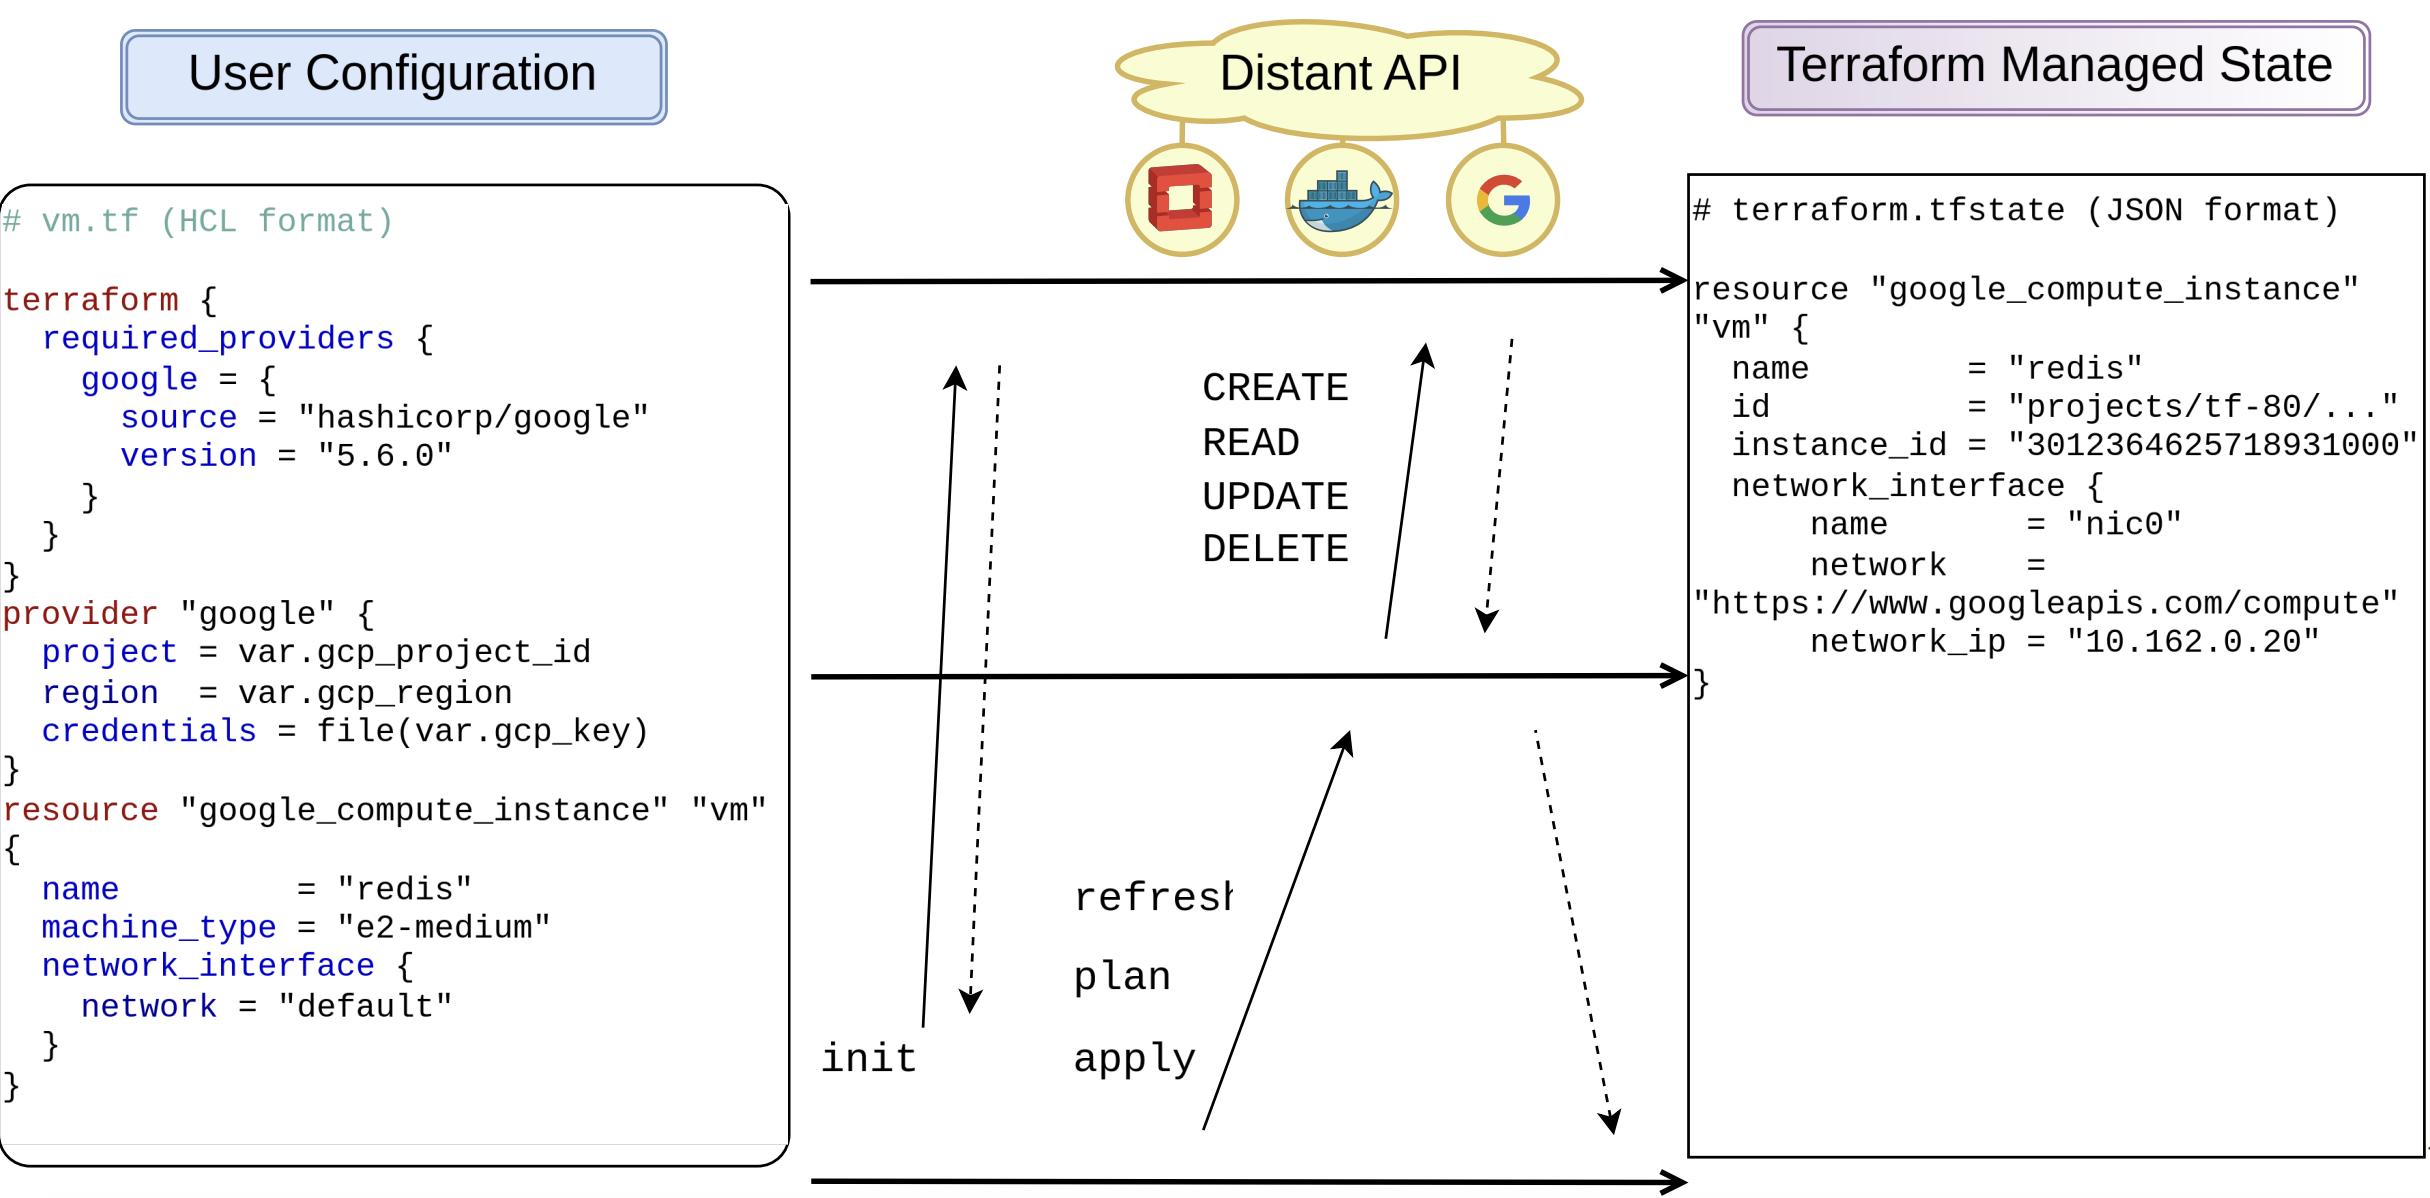
\includegraphics[scale=0.35]{figures/workflow}

\end{frame}

% -----------------
\section{Ecrire une configuration en HCL}
% -----------------

\begin{frame}{HCL: un langage de configuration déclaratif}

\begin{alertblock}{Définition en blocs}
En HCL, on définie des blocs, contenants des attributs sous la forme de clé-valeur. Un bloc peut lui même contenir un bloc. On parle alors de blocs imbriqués.
\end{alertblock}

\pause

\begin{alertblock}{Le bloc \lstinline[language=HCL]!terraform!}
Définit les paramètres globaux du projet Terraform :  
version requise, configuration du backend pour le \emph{state}, et gestion des providers.
\end{alertblock}

\pause

\begin{alertblock}{Le bloc \lstinline[language=HCL]!provider!}
Configure l'accès à un service cloud ou une API :  
informations de connexion, région, options spécifiques au fournisseur.
Ce bloc est nommé.
\end{alertblock}

\pause

\begin{alertblock}{Le bloc \lstinline[language=HCL]!resource!}
Décrit une ressource de l'infrastructure (VM, réseau, bucket...).  
Contient un type, un nom et des attributs configurables.
\end{alertblock}

\end{frame}

% -----------------

\begin{frame}{HCL: un langage de configuration déclaratif}

\begin{alertblock}{Attributs / Arguments / Champs}
Les attributs en HCL sont définis avec le signe \alert{égal} (\alert{=}).

La valeur des attributs peut être n'importe quelle expression: constante, appel de fonction, une liste, un objet, un référence, etc.

\begin{itemize}
    \item \lstinline[language=HCL]!name = "mon serveur"!
    \item \lstinline[language=HCL]!credentials = file("./creds.json")!
    \item \lstinline[language=HCL]!labels = \{app = "redis"\}!
    \item \lstinline[language=HCL]!image = docker\_image.redis.name!
    \item etc
\end{itemize}

\end{alertblock}

Les définitions \alert{multiples} d'un attribut sont \alert{interdites}. On ne fait qu'une seule attribution.

\end{frame}
% -----------------
\begin{frame}[fragile]{HCL: un langage de configuration déclaratif}

\begin{columns}[T]
  \begin{column}{0.55\textwidth}
    \begin{lstlisting}[language=HCL, basicstyle=\ttfamily\scriptsize]
terraform {
    required_providers {
        google = {
            source  = "hashicorp/google"   
            version = "5.6.0"
        }
    }
}
provider "google" {
    project = "mon_projet"
    region = "europe-west1"
    credentials = file(var.gcp_key)
}
resource "google_compute_instance" "vm" {
    name = "redis-${provider::google.project}"
    machine_type = "e2-medium"
    network_interface {
        network = "default"
    }
}
\end{lstlisting}
  \end{column}

  \begin{column}{0.45\textwidth}
    \begin{block}{Bloc \lstinline[language=HCL]!terraform!}
      \begin{itemize}
        \item Le bloc \lstinline[language=HCL]!terraform! définit des paramètres globaux.
        \item Ici, on indique que le provider utilisé est \texttt{google}.
        \item Le provider est téléchargé depuis le registry \texttt{hashicorp}.
        \item La version requise est fixée à \texttt{5.6.0}.
      \end{itemize}
    \end{block}
  \end{column}
\end{columns}

\end{frame}
% -----------------
\begin{frame}[fragile]{HCL: un langage de configuration déclaratif}

\begin{columns}[T]
  \begin{column}{0.55\textwidth}
    \begin{lstlisting}[language=HCL, basicstyle=\ttfamily\scriptsize]
terraform {
    required_providers {
        google = {
            source  = "hashicorp/google"   
            version = "5.6.0"
        }
    }
}
provider "google" {
    project = "mon_projet"
    region = "europe-west1"
    credentials = file(var.gcp_key)
}
resource "google_compute_instance" "vm" {
    name = "redis-${provider::google.project}"
    machine_type = "e2-medium"
    network_interface {
        network = "default"
    }
}
\end{lstlisting}
  \end{column}

  \begin{column}{0.45\textwidth}
    \begin{block}{Bloc \lstinline[language=HCL]!provider!}
    \begin{itemize}
\item \lstinline[language=HCL]!project = "mon_projet"! : identifiant du projet
\item \lstinline[language=HCL]!region = "europe-west1"! : région utilisée pour déployer les ressources.
\item \lstinline[language=HCL]!credentials = file(gcp_key.json)! : chemin vers la clé de service GCP
    \end{itemize}
    \end{block}
  \end{column}
\end{columns}

\end{frame}
% -----------------
\begin{frame}[fragile]{HCL: un langage de configuration déclaratif}

\begin{columns}[T]
  \begin{column}{0.55\textwidth}
    \begin{lstlisting}[language=HCL, basicstyle=\ttfamily\scriptsize]
terraform {
    required_providers {
        google = {
            source  = "hashicorp/google"   
            version = "5.6.0"
        }
    }
}
provider "google" {
    project = "mon_projet"
    region = "europe-west1"
    credentials = file(var.gcp_key)
}
resource "google_compute_instance" "vm" {
    name = "redis-${provider::google.project}"
    machine_type = "e2-medium"
    network_interface {
        network = "default"
    }
}
\end{lstlisting}
  \end{column}

  \begin{column}{0.45\textwidth}
    \begin{block}{Bloc \lstinline[language=HCL]!resource!}
\begin{itemize}
  \item \lstinline[language=HCL]!resource "..." "vm"! : définit une machine virtuelle avec l'id \lstinline[language=HCL]!vm!.
  \item \lstinline[language=HCL]!name = "redis-${provider::google.project}"! : le nom de la VM sera construit à partir de \emph{redis-} suivi du nom de projet dans le provider.
  \item \lstinline[language=HCL]!machine_type = "e2-medium"! spécifie le type de machine.
  \item \lstinline[language=HCL]!network_interface { network = "default" }!  rattache l’instance au réseau par défaut.
\end{itemize}
    \end{block}
  \end{column}
\end{columns}
\end{frame}


\begin{frame}{HCL: un langage de configuration déclaratif}

Quelques autres blocs

\begin{alertblock}{Le bloc \lstinline[language=HCL]!data!}
Permet de récupérer des informations existantes depuis un provider. Le contenu est en \alert{lecture-seule}.
\end{alertblock}

\begin{alertblock}{Le bloc \lstinline[language=HCL]!module!}
Regroupe plusieurs ressources et variables dans une unité réutilisable.  
Facilite la \alert{factorisation} et la \alert{réutilisation} du code Terraform.
Un fichier \textbf{.tf} est lui même un module.
\end{alertblock}

\begin{alertblock}{Le bloc \lstinline[language=HCL]!check!}
Permet de définir des conditions de validation dans la configuration.  
Terraform échoue si la condition n’est pas respectée $\Rightarrow$ utile pour garantir des \alert{contraintes métiers}.
\end{alertblock}

\begin{alertblock}{Le bloc \lstinline[language=HCL]!import!}
Relie une ressource réelle déjà existante dans le cloud à une ressource définie dans le code Terraform.  
\alert{Important} : permet d’intégrer de l’infra existante sans la recréer.
\end{alertblock}

\end{frame}

% -----------------

\begin{frame}{HCL: un langage de configuration déclaratif}
    
    \begin{alertblock}{Variables}
        Les modules peuvent avoir \alert{trois types} de variables:
        \begin{itemize}
            \item Inputs
            \item Outputs
            \item Locals
        \end{itemize}  
        Ces variables sont définies avec les blocs:  \lstinline[language=HCL]!variable!, \lstinline[language=HCL]!output! et  \lstinline[language=HCL]!locals!.
    \end{alertblock}

\end{frame}

% -----------------

\begin{frame}{HCL: un langage de configuration déclaratif}

 \begin{alertblock}{Références}
    \begin{itemize}
        \item Les attributs d'une ressource sont référencées par le \alert{type} et le \alert{nom} de la ressource, suivi du nom de la ressource. Par exemple: \lstinline[language=HCL]!docker\_image.redis.image\_id!
        \item Pour référencer depuis un bloc \lstinline[language=HCL]!data!, on utilise le mot clé \lstinline[language=HCL]!data!. Par exemple: \lstinline[language=HCL]!data.docker\_image.redis.image\_id!
        \item Pour les variables de type \emph{input} et \emph{local}, on utilse les mots clés \lstinline[language=HCL]!var! et \lstinline[language=HCL]!local!. Par exemple: \\
        \lstinline[language=HCL]!var.my\_input\_var! \\ \lstinline[language=HCL]!local.my\_local\_var!
    \end{itemize}       

    \end{alertblock}

\end{frame}

% -----------------

\begin{frame}[fragile]{HCL: un langage de configuration déclaratif}

\begin{columns}[T]
  \begin{column}{0.43\textwidth}
    \begin{lstlisting}[language=HCL, basicstyle=\ttfamily\scriptsize]
terraform {
  required_providers {
    google = {
      source  = "hashicorp/google"
      version = "5.6.0"
    }
  }
}

provider "google" {
  project = "my-gcp-project-id"
  region  = "europe-west1"
  credentials = file(gcp_key.json)
}

data "google_compute_image" "debian" {
  family  = "debian-11"
  project = "debian-cloud"
}

locals {
  prefix = "app"
}
\end{lstlisting}
\end{column}

\begin{column}{0.57\textwidth}
\begin{lstlisting}[language=HCL, basicstyle=\ttfamily\scriptsize]
resource "google_compute_instance" "redis" {
  name = "redis-01"
  machine_type = "e2-micro"
  boot_disk {
    initialize_params {
      image = data.google_compute_image.debian.self_link
    }
  }
  network_interface {
    network = "default"
    access_config {}
  }
}
resource "google_compute_instance" "app" {
  name = "${local.prefix}-${google_compute_instance.redis.name}"
  machine_type = "e2-medium"
  boot_disk {
    initialize_params {
      image = data.google_compute_image.debian.self_link
    }
  }
  network_interface {
    network = "default"
    access_config {}
  }
}
\end{lstlisting}
\end{column}
\end{columns}
\end{frame}

% -----------------

% -----------------
\section{Quelques bonnes pratiques}
% -----------------

\begin{frame}{Convention de nommage}

Un code d'IaC est aussi source de documentation.

\begin{alertblock}{Bonne pratique 1}
\begin{itemize}
    \item Donner toujours une description de la ressource au sein de son nom
    \begin{itemize}
        \item Environnement
        \item Type de la ressource 
        \item But, usage, intention
        \item Exemple: \texttt{\textbf{dev-firewall-rule-allow-helloworld-to-database}}
    \end{itemize}
\end{itemize}
\end{alertblock}
\end{frame}

% -----------------

\begin{frame}{Variables et constantes}

\begin{alertblock}{Bonne pratique 2}
\begin{itemize}
    \item De manière générale: Privilégiez les constantes plutôt que les variables
    \item Si le changement d'une valeur affecte les dépendances de l'infrastructure ou compromets des informations sensibles, utilisez une variable
\end{itemize}
\end{alertblock}

\end{frame}

\begin{frame}{Avoid troubleshooting}

\begin{alertblock}{Bonne pratique 3}
\begin{itemize}
    \item Bien lire et comprendre chaque déclarations et le plan avant de faire un \texttt{terraform apply}
    \item Versionner le code Terraform, sans commit de secrets
    \item Intégrer du CI/CD sur votre infrastructure Terraform
    \item Stocker vos fichiers d'état (.tfstate) sur des stockages distants avec des mecanismes de lock
\end{itemize}
\end{alertblock}

\end{frame}

\end{document}
